\documentclass[a4paper,12pt,onecolumn]{article}
\usepackage[utf8]{inputenc}
\setlength{\columnsep}{1cm}
\usepackage[utf8]{inputenc}
\usepackage[brazil]{babel}
\usepackage{amsmath}
\usepackage{bbm}
\numberwithin{equation}{section}
\numberwithin{figure}{section}
\usepackage{hyperref}
\usepackage{graphicx}
\usepackage[stable]{footmisc}
\usepackage{xcolor,colortbl}
\addtolength{\hoffset}{-0.5cm}
\addtolength{\textwidth}{1.5cm}
\usepackage{bigints}
\usepackage{comment}
\usepackage{indentfirst}
\usepackage{abstract}
\renewcommand{\abstractnamefont}{\normalfont\Large\bfseries}
\renewcommand{\abstracttextfont}{\normalfont}
\usepackage{float}

\begin{document}

\begin{figure}[hbtp]
\centering
\includegraphics[scale=0.5]{ufabc.jpg}
\end{figure}

\begin{center}
{\large \textbf{Universidade Federal do ABC}}
\end{center}
\begin{center}
{\scriptsize CENTRO DE ENGENHARIA, MODELAGEM E CIÊNCIAS SOCIAIS APLICADAS - CECS}
\end{center}

\vspace{1cm}

\hrule
\begin{center}
\textbf{Experimento 2 - Medidas de sinais senoidais em circuito RC}
\end{center}
\hrule

\vspace{2cm}

\begin{center}
\begin{tabular}{lc}
Gabriel Moraes de Souza     &   \textbf{RA: 11201811286} \\
Giuliano Busatto Perasolo   &   \textbf{RA: 11201811787} \\
Lucas Moura de Almeida       &  \textbf{RA: 11201811415} \\
Pedro Henrique Assarito Araújo &\textbf{RA: 11201810768} \\
Rafael Balaguer Soares      &   \textbf{RA: 11201810153} \\
\end{tabular}
\end{center}

\vspace{2cm}

\begin{center}
São Bernardo do Campo - 2020
\end{center}

\newpage
\begin{abstract}
%Resumo: Breve texto sobre os objetivos do experimento, metodologia utilizada, principais resultados e Conclusões
O presente experimento tem o propósito de estudar, analisar e discutir um circuito RC série. De modo que é capaz de nos proporcionar um alto nível de entendimento do funcionamento de um capacitor e familiarização com osciloscópio. Visto que é necessário tratar de uma fonte de corrente alternada, ou seja, formas de ondas senoidais, é altamente necessário compreender os chamados fasores, portanto inserindo como objeto de estudo os números complexos.
\end{abstract}

\newpage
\begin{center}
\tableofcontents
\end{center}

\newpage
\section{Introdução}
%Descrição experimental e Metodologia: Fluxograma do procedimento utilizado, ressaltando detalhes experimentais observados em laboratório (e que não estejam contidos no roteiro)
Um circuito RC é composto por um conjunto de resitores e capacitores que por sua vez podem ser simplificados somente por um resistor equivalente e um capacitor equivalente, ao se aplicar as fórmulas para resistores em série \ref{req_s}, resistores em paralelo \ref{req_p}, capacitores em série \ref{ceq_s} e capacitores em paralelo \ref{ceq_p}. De modo que o circuito pode ser representado como é mostrado na figura \ref{c1}, com forma simplificada que será utilizado em nosso experimento e que posteriormente haverá uma análise mais criterioza.

\begin{equation}
R_{s} = \sum_{i=1}^{\infty} R_{i}
\label{req_s}
\end{equation}

\vspace{0.5cm}

\begin{equation}
\dfrac{1}{R_{p}} = \sum_{i=1}^{\infty} \dfrac{1}{R_{i}}
\label{req_p}
\end{equation}

\vspace{0.5cm}

\begin{equation}
\dfrac{1}{C_{s}} = \sum_{i=1}^{\infty} \dfrac{1}{C_{i}}
\label{ceq_s}
\end{equation}

\vspace{0.5cm}

\begin{equation}
C_{p} = \sum_{i=1}^{\infty} C_{i}
\label{ceq_p}
\end{equation}

\vspace{0.5cm}

\begin{figure}[H]
\centering
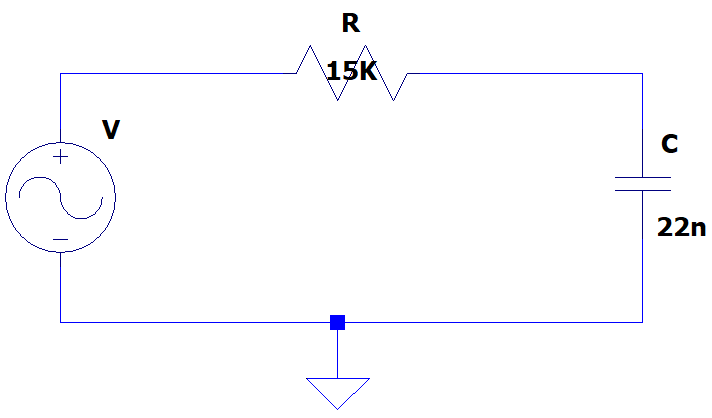
\includegraphics[scale=0.5]{c1.png}
\caption{Esquema simplificado do circuito RC }
\label{c1}
\end{figure}

Haja visto a breve explicação anterior, este experimento pode ser inicialmente descrito de maneira simplificada e adequada através de um fluxograma, apresentado na figura \ref{flux}, assim detalhando passo a passo os procedimentos realizados em sua execução.

\begin{figure}[H]
  \centering
  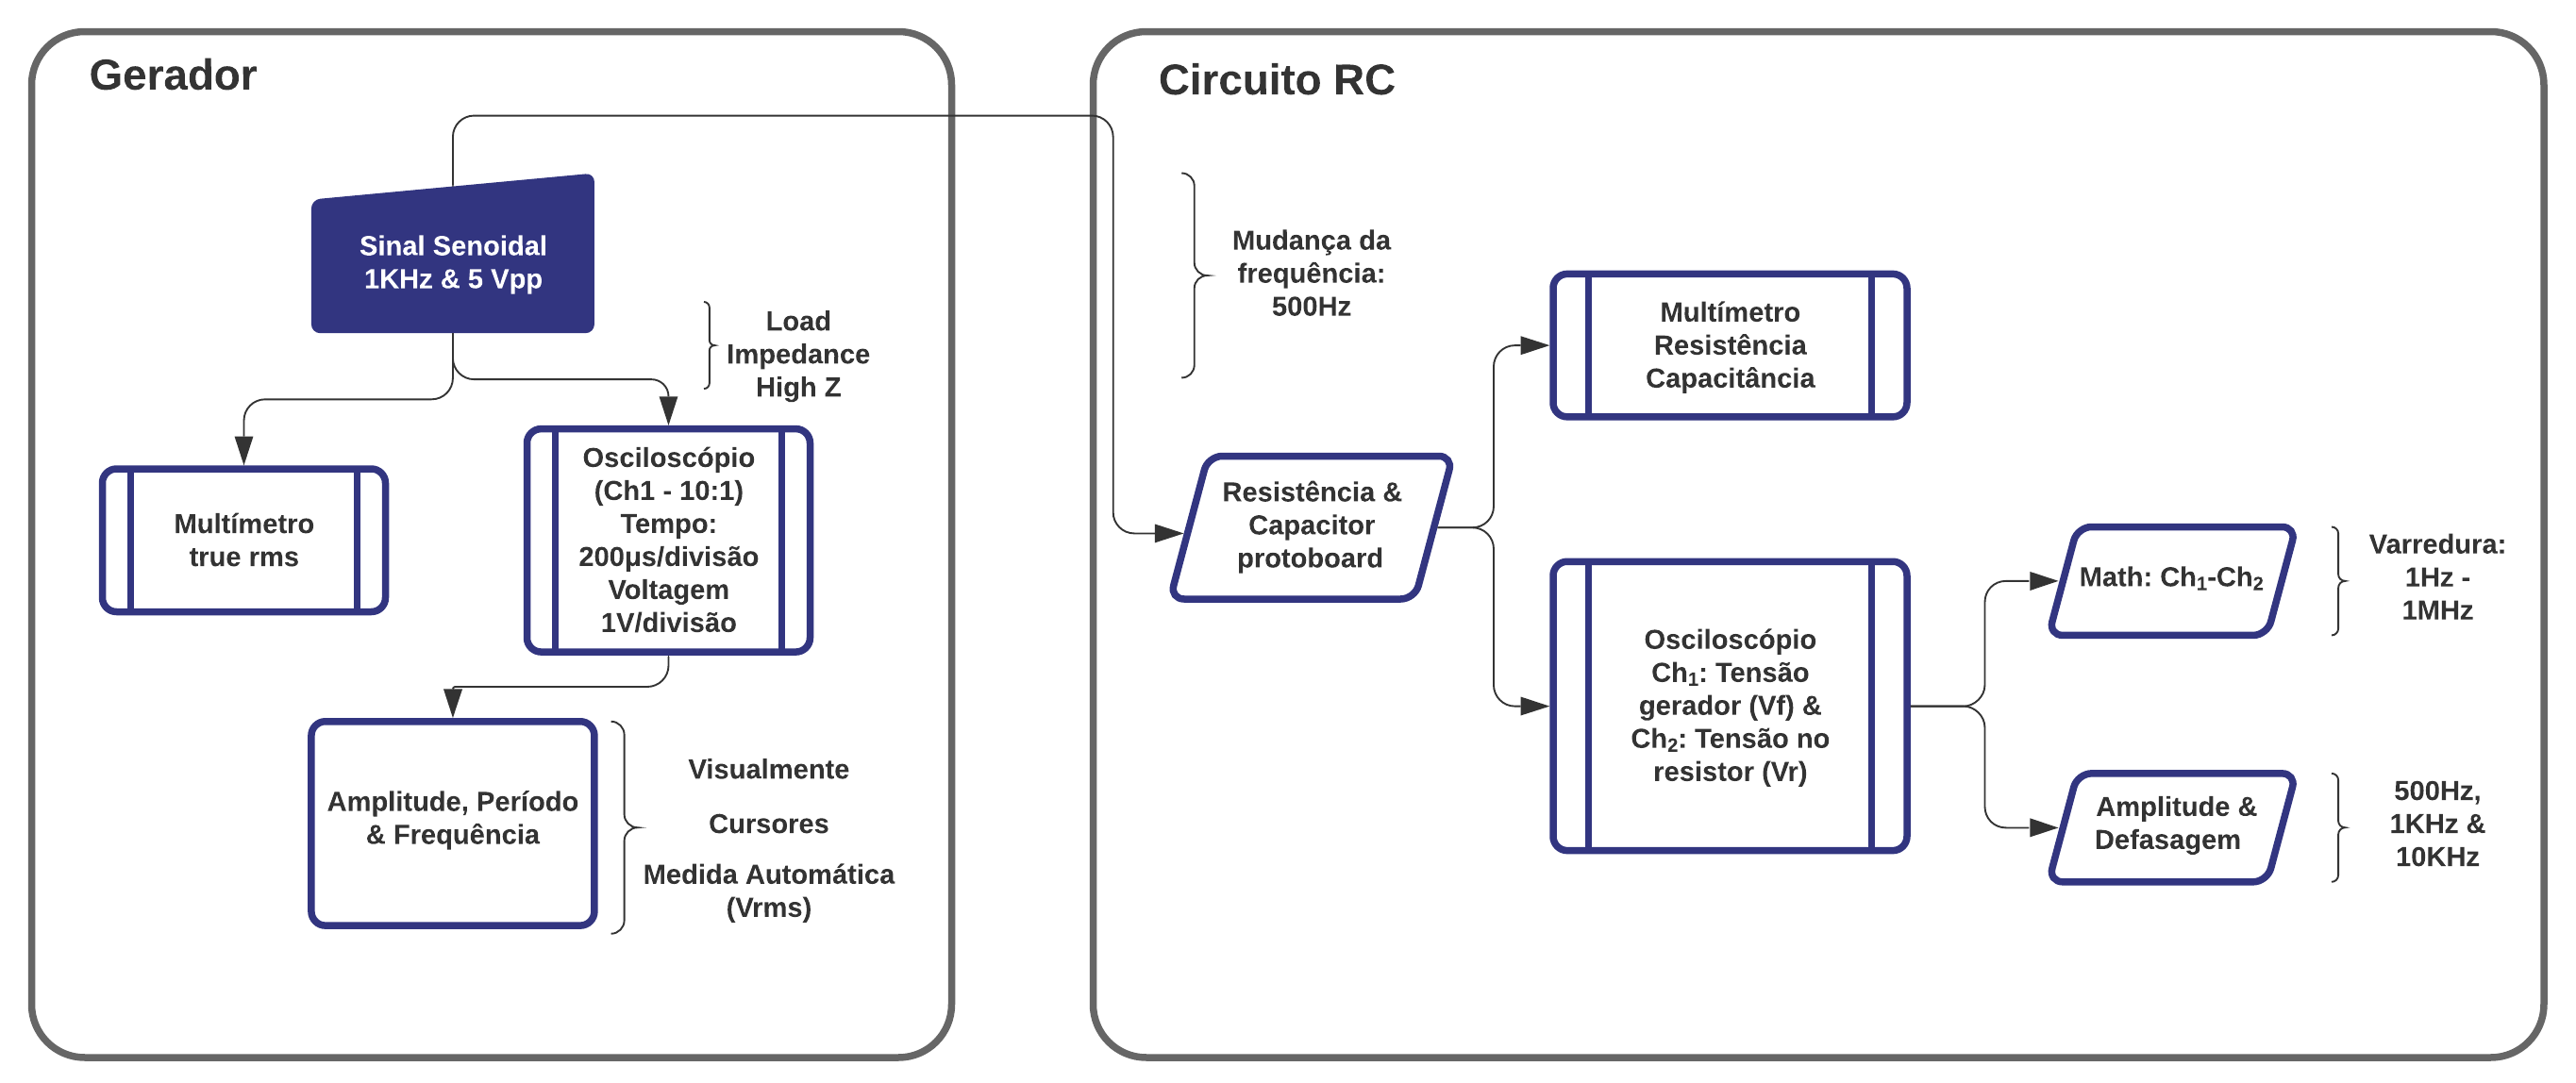
\includegraphics[scale=0.65]{fluxograma.png}
  \caption{Fluxograma descritivo do experimento}
  \label{flux}
\end{figure}


\newpage
\section{Dados experimentais e resultados}
%Dados experimentais e resultados: Tabelas com dados coletados em laboratório, acompanhados de respectiva incertezas. Tabelas e gráficos com os resultados medidos e calculados
\subsection{Gerador}
Primeiramente no início do experimento é necessário realizar certos ajustes e medições para que se inicie o estudo do circuito proposto. O gerador Tektronix AFG3021B, representado na figura \ref{ger}, é ajustado  de modo a gerar um sinal senoidal de $10^{3}$ Hz, uma tensão pico a pico ($V_{pp}$) de 5V e necessário ajustar a resitência de carga "Load Impedance" para "High Z".

\begin{figure}[H]
  \centering
  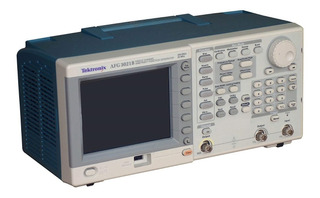
\includegraphics[scale=0.6]{ger.png}
  \caption{Gerador Tektronix AFG3021B}
  \label{ger}
\end{figure}

O sinal gerado é finalmente inserido canal 1 do osciloscópio Tektronix TDS2024C, representado na figura \ref{osc}, sendo este ajustado com a configuração da ponta de prova (10:1) e para tanto foi utilizado o menu do dispositivo.

\begin{figure}[H]
  \centering
  \includegraphics[scale=0.6]{oscil.png}
  \caption{Osciloscópio Tektronix TDS2024C}
  \label{osc}
\end{figure}

Outro passo essêncial foi o de ajustar a base de tempo para $250 \mu s$ por divisão assim como a voltagem para 1V por divisão. Através da figura \ref{osc1} podemos observar 2.5 periodos na tela.

\begin{figure}[H]
  \centering
  \includegraphics[scale=0.25]{oscil1.jpeg}
  \caption{Inserção do sinal gerado no canal 1}
  \label{osc1}
\end{figure}

Com base no que foi realizado até o momento é preciso realizar a medição da amplitude ($V_{pp}$), do período P e da frequência f de três formas distintas:

\begin{itemize}
\item Visualmente com o uso da divisões pré estabelecidass
\item Utilizando os cursores presente no osciloscópio
\item Utilizar o recurso de medida automática paraa obter o valor eficaz ($V_{rms}$)
\end{itemize}

%TABELA COM OS VALORES  AQUI !!!!!!!!!!!!!!	

Por fim medimos o sinal de saída do gerador utilizando o múltimetro de bancada presente. Como é mostrado na figura .... obtemos o valor de ... que representa o $V_{rms}$ 

%INSERIR INCERTEZAS !!!!!!!!!!!!

\subsection{Circuito RC}
Inicialmente foram medidos os valores da capacitância e resistência dos componentes, possuindo os valores de......, presentes para montagem do circuito em uma protoboard, figura....

%FOTO DA PROTOBOARD

O sistema esquematico da figura.... foi fielmente representado por um sistema real 

%FOTO DO CIRCUITO C2

Ajustar 500hz e vpp = 5V Load impedance para highz 
ponta de prova 1 - tensao gerada Vf
ponta de prova 2 - tensao no resistor Vr
Simultaneo na tela do osciloscopio

Utilize a função MATH para realizar Ch1-Ch2 para obter a tensao no capacitor Vc

Varredura 1hz - 1Mhz
Observe as formas de onda obtidas bem como Ch1-Ch2 Observe o que ocorre ao variar a frequencia

Ajuste a frequencia do gerador de volta para 500hz

Meça amplitude dos 3canais e defasagem do sinal do canal 2 em relação ao sinal do canal 1 (NOTA)
Refaça o anterior para 1khz  e 10khz



\newpage
\section{Interpretação dos resultados}
%Interpretação dos resultados: Resposta às questões propostas, com respectivas justificativas


\newpage
\section{Discussão e conclusões}
%Discussão e conclusões: Análise crítica do experimento e dos resultados. Ressaltar os conceitos teóricos que foram testados em laboratório	e os conhecimentos extras adquiridos (sobre os componentes e equipamentos utilizados)


\newpage
\section{Referências bibliográficas}

\newpage
\section{Anexo}
\subsection{Cálculo das incertezas}



\end{document}
